\documentclass{beamer}
\usepackage[utf8]{inputenc}
\usepackage[T1]{fontenc}
\usepackage[polish]{babel}
\usepackage{graphicx}
\usepackage{times}

\usetheme{AGH}

\title[Biometryczny System Kontroli Dostępu]{Biometryczny System Kontroli Dostępu}

\author[T. Drzewiecki, J. Gajda]{Tomasz Drzewiecki, Joanna Gajda}

\date[2012]{9.01.2012}

\institute[AGH-EAIE]
{Wydział Elektrotechniki, Automatyki, Informatyki i Elektroniki\\ 
Katedra Automatyki
}

\setbeamertemplate{itemize item}{$\maltese$}

\begin{document}

{
%\usebackgroundtemplate{
\includegraphics[width=\paperwidth]{titlepage}} % wersja angielska
\usebackgroundtemplate{
\includegraphics[width=\paperwidth]{titlepagepl}} % wersja polska
 \begin{frame}
   \titlepage
 \end{frame}
}

%---------------------------------------------------------------------------

\begin{frame}
\frametitle{Tematyka projetku}

\begin{block}{Cel projektu}
Celem naszego projektu było stworzenie/rozbudowa systemu do identyfikacji osób na podstawie tęczówki oka.
\end{block}

\begin{figure}
\begin{center}
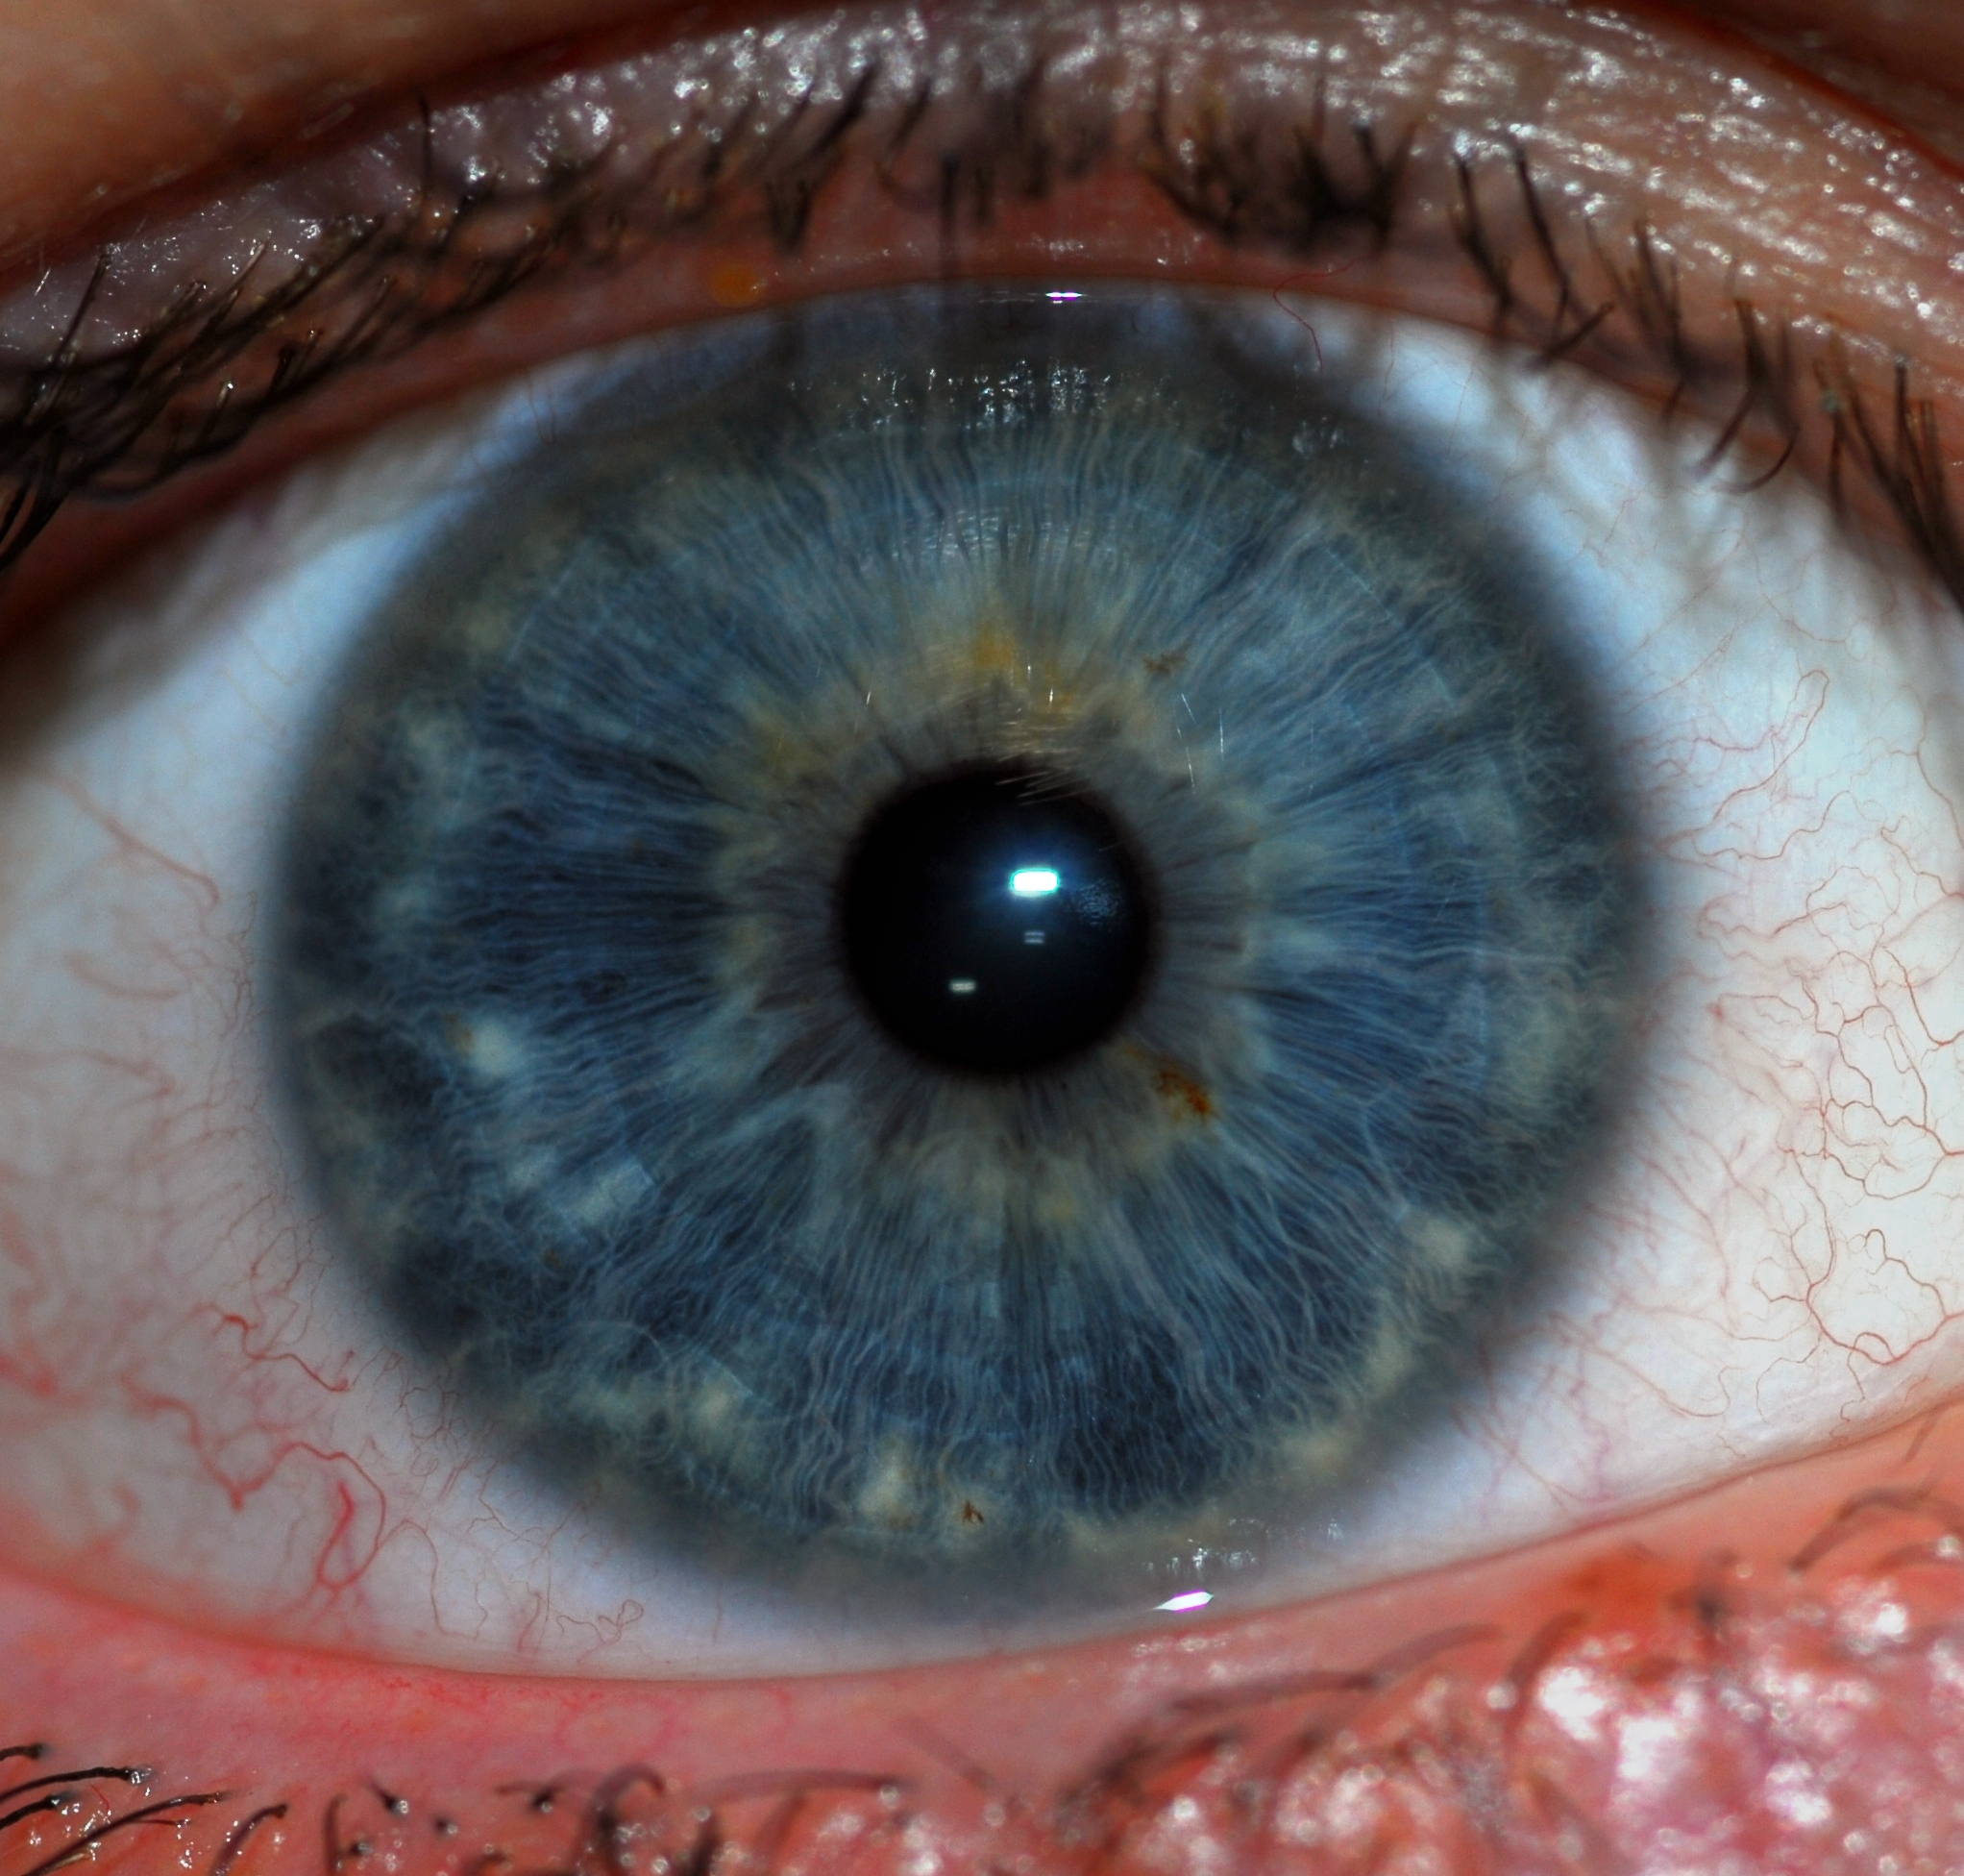
\includegraphics[scale=0.04]{teczowka.jpg}
\caption{Tęczówka człowieka}
\end{center}
\end{figure}

\end{frame}

%---------------------------------------------------------------------------

\begin{frame}
\frametitle{Podział systemu}

Tworzony przez nas system składa się z trzech głównych cześci:
\begin{columns}[t]
\column{0.3\textwidth}
\begin{block}{Część sprzętowa}
Odpowiedzialna za pobranie obrazu tęczówki od badanych osób. Najważniejszym elementem jest kamera oraz zapewnienie odpowiednich warunków.
\end{block}
\column{0.3\textwidth}
\begin{block}{Cześć biometryczna}
Część odpowiedzialna na zamianę obrazu tęczówki na kod tęczówki oraz późniejsze porównywanie utworzonych kodów.
\end{block}
\column{0.3\textwidth}
\begin{block}{Część bazodanowa}
Część odpowiedzialna za przechowywanie danych osób wprowadzanych do systemu.
\end{block}
\end{columns} 

\end{frame}

%---------------------------------------------------------------------------

\begin{frame}
\frametitle{Konstrukcja stanowiska}
Stanowisko do pobierania obrazów musi spełniać odpowiednie wymagania. Im lepsze będą pobierane obrazy, tym łatwiejsza będzie późniejsza segmentacja. Główne założenia:
\begin{itemize}
\item Likwidacja odblasków pochodzących z oświetlenia (naturalnego oraz sztucznego),
\item Odpowiednia jasność obrazu,
\item Odpowiednia jakość obrazu,
\item Odpowiednia wielkość tęczówki na obrazie.
\end{itemize}
\end{frame}
%---------------------------------------------------------------------------

\begin{frame}
\frametitle{Konstrukcja stanowiska}
Udało się skonstruować stanowisko spełniające wymagania:
\begin{itemize}
\item Odblaski usunięto poprzez zasłonięcie źródeł światła (za pomocą kartonowego pudła),
\item Odpowiednią jasność zapewnia oświetlacz IR,
\item Odpowiednią jakość obrazu zapewnia odpowiednia kamera, która potrafi rejestrować obrazy w dużej rozdzielczości,
\item Odpowiednią wielkość tęczówki otrzymujemy stosując przybliżenie za pomocą obiektywu.
\end{itemize}
\end{frame}

%---------------------------------------------------------------------------

\begin{frame}
\frametitle{Stworzone stanowisko}
Kilka zdjęć
\begin{figure}
\begin{center}
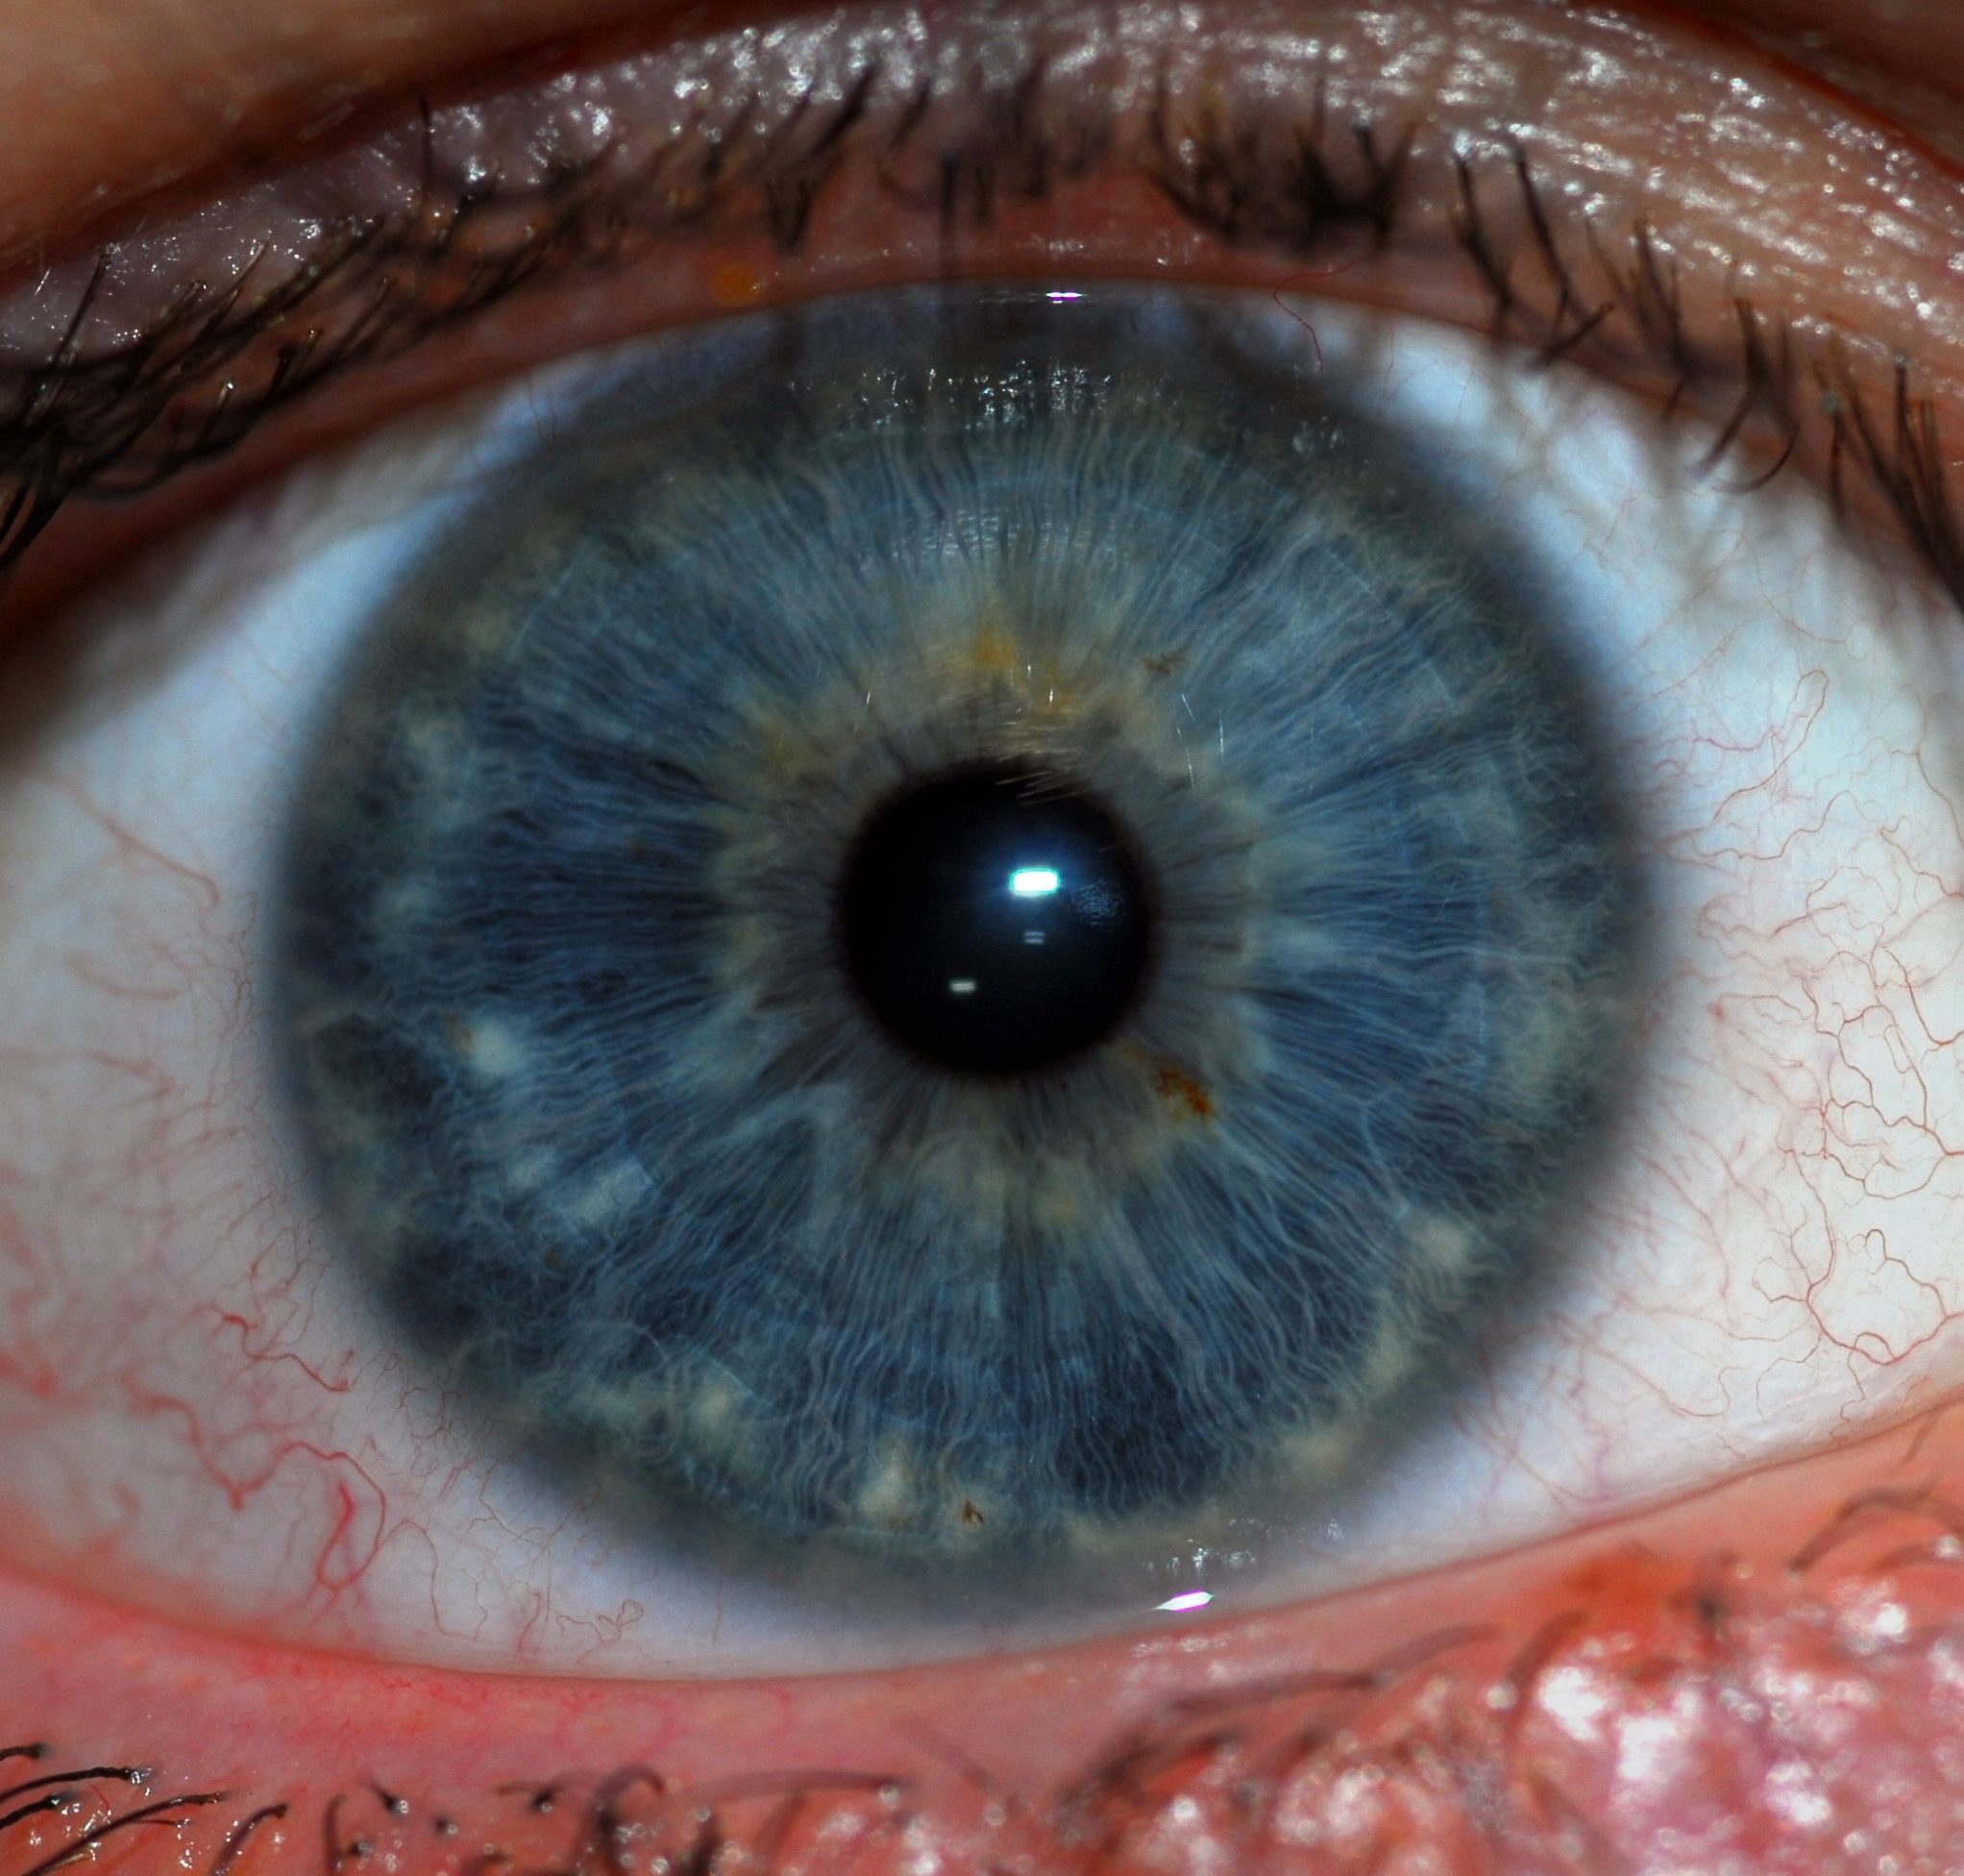
\includegraphics[scale=0.04]{stanowisko.jpg}
\end{center}
\end{figure}
\end{frame}

%---------------------------------------------------------------------------

\begin{frame}
\frametitle{Algorytm do tworzenia kodu tęczówki}
\begin{figure}
\begin{center}
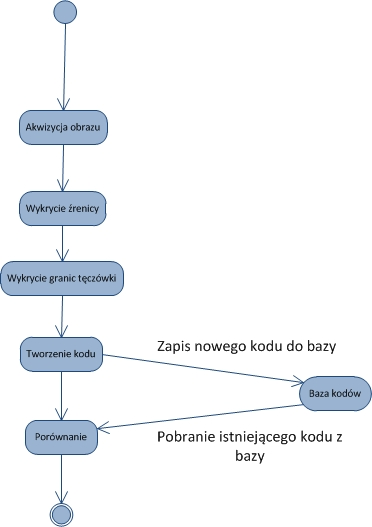
\includegraphics[scale=0.4]{schemat.jpg}
\end{center}
\end{figure}
\end{frame}

%---------------------------------------------------------------------------

\begin{frame}
\frametitle{Wykrycie źrenicy}
Celem tej części algorytmy jest opisanie źrenicy jako okrąg, czyli znalezienie środka okręgu na obrazie oraz jego promienia. Punktem startowym jest pobrany obraz z kamery.
\begin{figure}
\begin{center}
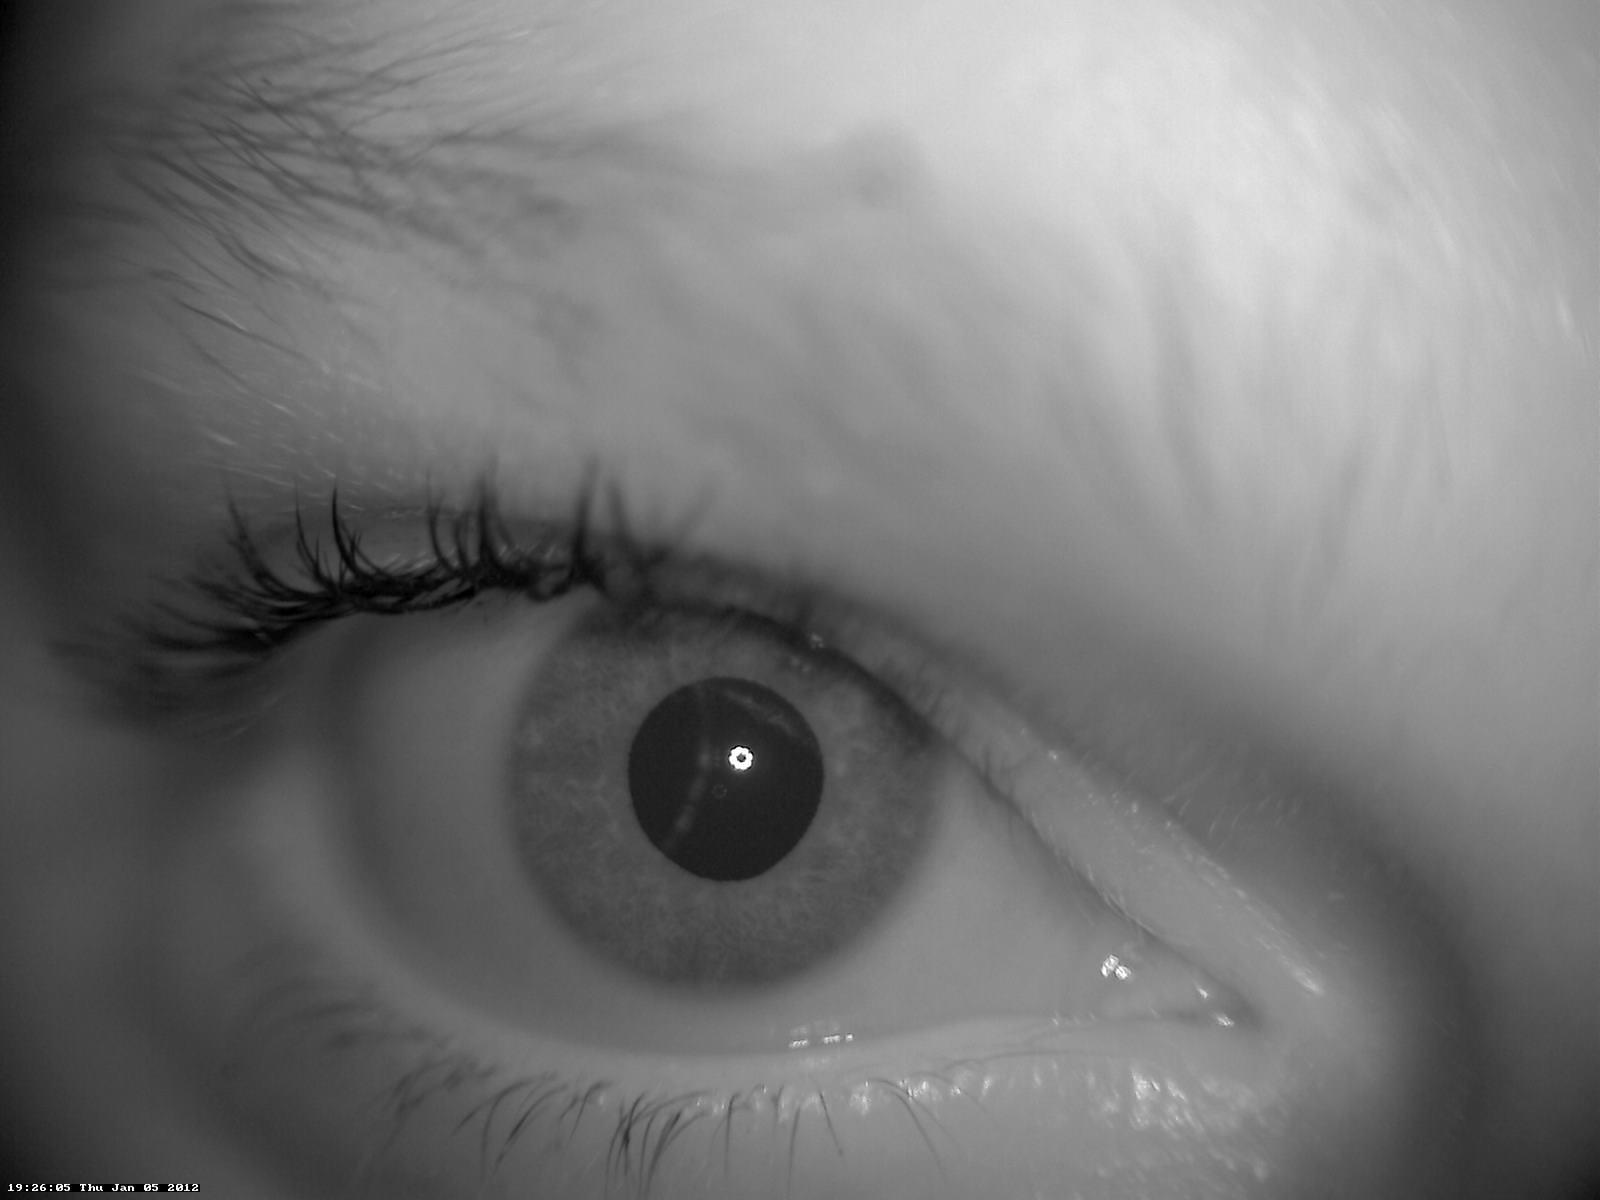
\includegraphics[scale=0.13]{szarosc.jpg}
\end{center}
\end{figure}
\end{frame}

%---------------------------------------------------------------------------

\begin{frame}
\frametitle{pusty slajd}

\end{frame}

%---------------------------------------------------------------------------

\begin{frame}
\frametitle{pusty slajd}

\end{frame}

%---------------------------------------------------------------------------

\begin{frame}
\frametitle{Koniec}

\begin{block}{}
Dziękujemy za uwagę.\\
Pytania?
\end{block}


\end{frame}

%---------------------------------------------------------------------------


\end{document}

